\section{Reliability, Resources, and Operation}
\label{sec:operations}\label{sec:execution}\label{sec:reliability}\label{sec:workbench}\label{sec:deploy}

\begin{designbox}
Treat execution drift --- not weak reasoning --- as the primary risk of a multi-hour
run. Every degradation mode maps to a named guard that fails soft and is precise
about whether it may interrupt a live call. Route every provider call through one
priced, reservation-backed gateway so spend is bounded and attributable. Give the
operator a live, authenticated cockpit over the same tape, and deploy as a standard
service that drains cleanly.
\end{designbox}

The reliability model is a set of guards that keep a mission bounded and honest.
Figure~\ref{fig:reliability} sketches how they wrap one Engineer/Reviewer loop over a
persistent budget, event-log, and artifact rail. None of these guards decides whether
the research is good: each enforces a task-agnostic invariant and fails soft ---
reliability is added \emph{around} the agent's judgment, never in place of it.

\begin{figure}[ht]
\centering
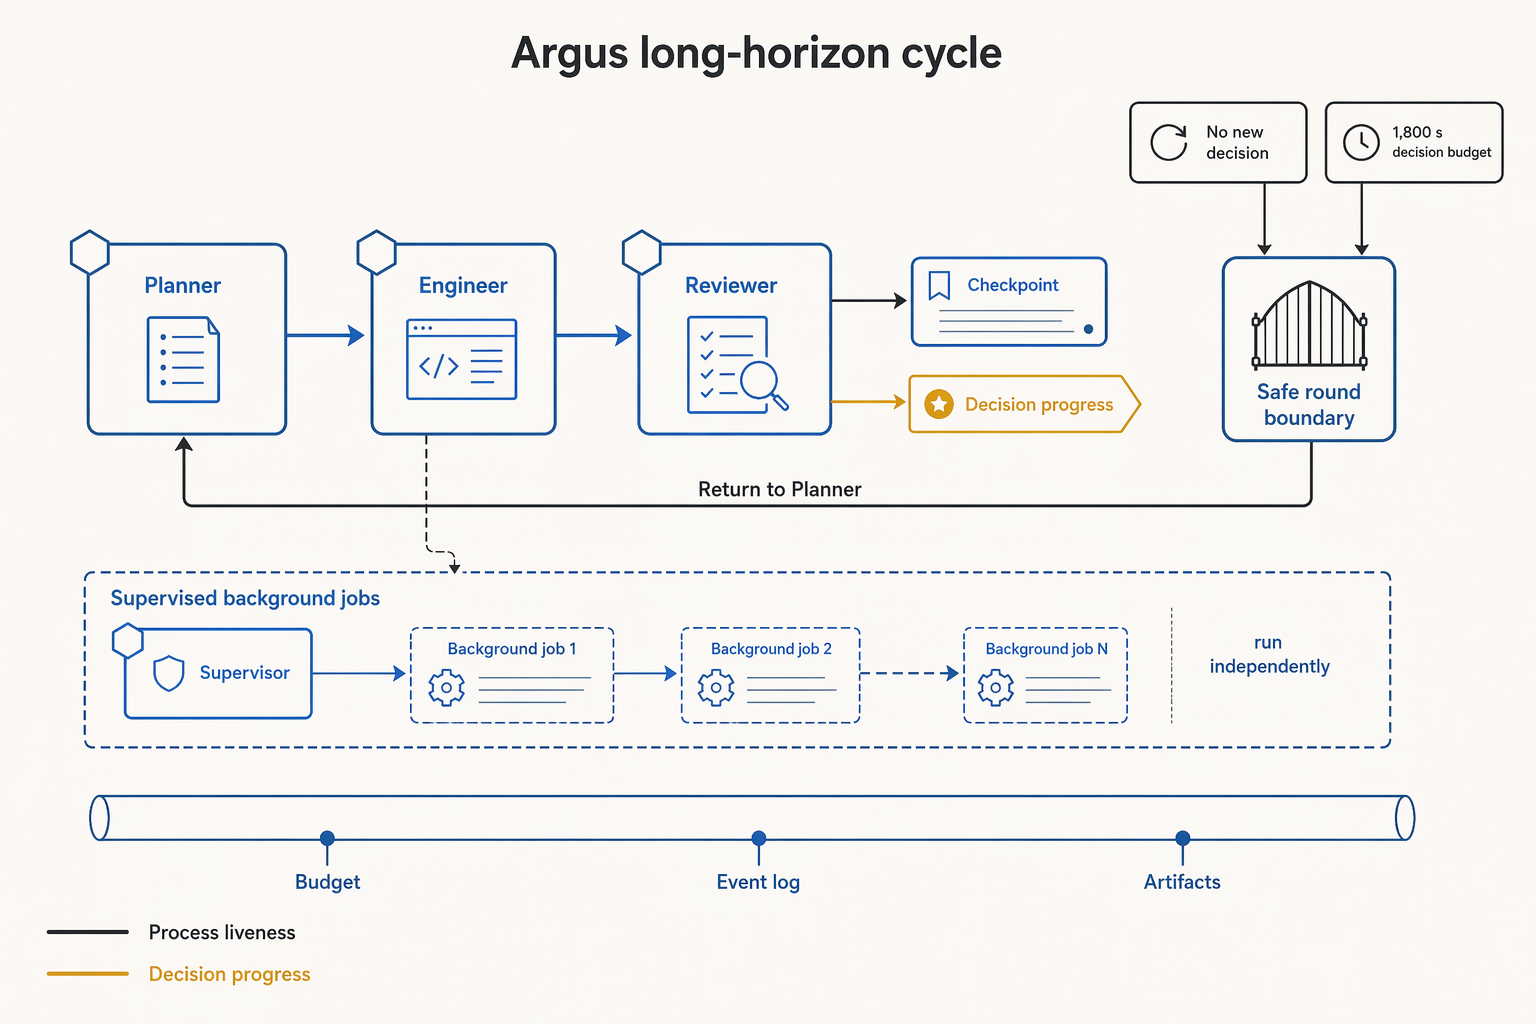
\includegraphics[width=0.6\textwidth]{figures/long_horizon_reliability.png}
\caption{System schematic (not a measured performance plot) of the long-running
reliability cycle: Planner, Engineer, and Reviewer run one loop; the Reviewer
maintains a bounded curated checkpoint and a decision-progress class that guides the
next Engineer round; supervised background jobs run alongside; and a safe round
boundary returns a stalled or budget-exhausted mission to the Planner.}
\label{fig:reliability}
\end{figure}

\subsection{Decision progress, not activity}

To separate real progress from busy churn, the Reviewer labels each round with a
\code{progress\_class}: \code{decision} or \code{evidence} for genuine forward
motion, or \code{setup\_only}, \code{artifact\_sync\_only}, or \code{none} for
nondecision work. The runtime \emph{counts} these structured labels; it never infers
progress from tool activity, filenames, or token emission. Four consecutive
nondecision rounds trip the stall guard, and a 1,800-second decision-progress
budget --- measured from the last decision or evidence increment and checked only
between rounds --- ends a mission that is spinning without ever cutting useful
in-flight work. A separate soft/hard round escalation (12/24) catches the rarer case
of a mission that makes evidence progress every round but never passes its gate,
asking the Reviewer to return \code{blocked} and, failing that, force-ending so the
Planner re-plans. Table~\ref{tab:guards} is the full guard matrix.

\begin{table}[h]
\centering
\small
\begin{tabularx}{\linewidth}{@{}p{2.7cm} X p{1.35cm} p{1.9cm}@{}}
\toprule
\textbf{Guard} & \textbf{Trigger \; / \; action} & \textbf{Default} & \textbf{Interrupts live call?} \\
\midrule
Backend-failure recovery & failure streak $\rightarrow$ backoff, then end as error & 2 / 15\,s & no (round boundary) \\
No-progress bail & consecutive rounds with no engineer message & 2 & no \\
Decision stall & consecutive nondecision \code{progress\_class} rounds $\rightarrow$ end & 4 & no \\
Decision-progress budget & seconds since last decision/evidence $\rightarrow$ end & 1{,}800\,s & \textbf{no} \\
Soft round escalation & round index $\rightarrow$ ask Reviewer to return \code{blocked} & 12 & no \\
Hard round escalation & round index $\rightarrow$ force-end as \code{blocked} & 24 & no \\
Effective-progress watchdog & no file change / non-token event $\rightarrow$ kill subprocess & 3{,}600\,s & \textbf{yes} \\
Runner hard-idle & no runner activity $\rightarrow$ interrupt round & 3{,}600\,s & \textbf{yes} \\
In-round compaction limit & auto-compactions within one round $\rightarrow$ end round & 3 & \textbf{yes} \\
\bottomrule
\end{tabularx}
\caption{Reliability guards (\code{engineer/runner.py}). Round-boundary guards never
sever a live call; the three in-round guards fire only against a subprocess emitting
token noise or looping without effective progress. All are env-overridable and
disable at 0.}
\label{tab:guards}
\end{table}

\subsection{In-round watchdogs and backend failure}

Three guards operate \emph{inside} a round because they target a subprocess that has
stopped doing useful work. The effective-progress watchdog kills a provider
subprocess that keeps emitting heartbeat or token noise for 3,600 seconds with no
file change and no non-token session event; the runner hard-idle watchdog interrupts
a round with no runner activity at all; and the in-round compaction guard ends a
round whose session auto-compacts three times. Each default is intentionally long ---
research turns legitimately spend many minutes reading, planning, or waiting on
model-side recovery --- and each disables at 0. A backend failure streak triggers a
bounded backoff and, if it persists, ends the mission as an error. A degraded reviewer
backend is routed to the structured \code{backend\_unavailable} status --- treated as
infrastructure and never as a \code{continue} --- after a historical blind-gate
incident in which a stale import-time schema path ran the completion gate blind for
roughly ninety minutes; the reviewer now preflights its schema file and raises if it
is unreadable rather than proceeding blind.

\subsection{One gateway, pricing, and budget reservations}

All backend execution flows through a single application-level gateway,
\code{RunExecGateway.execute} (\srcpath{core/run\_gateway.py}). Token usage is priced
by a small module (\srcpath{core/pricing.py}, default model \code{gpt-5.5}) and
accumulated in a \emph{presence-aware} usage ledger (\srcpath{core/usage.py}) that
distinguishes a genuine zero from omitted usage, so no cost is ever fabricated from
missing data. Spend control is reservation-based and event-backed: before a call runs
the runtime creates a budget reservation, recorded as one of
\code{budget.reservation.created}, \code{.denied}, \code{.settled}, or
\code{.released}, with \code{budget.unpriced.blocked} and
\code{budget.fence\_breach.blocked} for the unpriceable or fence-breaching cases. This
reservation-then-reconciliation cycle --- settle on completion, release on abort ---
keeps the ledger honest, and the provider-side spend fences on a call
(\code{max\_budget\_usd}, \code{max\_ai\_credits}) are injected from the reservation,
not from role configuration, so a role cannot raise its own ceiling. The principal
live defaults, resolved once for the CLI, daemon, and Web launch paths by the
canonical \code{resolve\_budget\_caps} knob resolver (\srcpath{core/knobs.py}), are a
per-mission preflight cap of \$30, a daily cap of \$180, a global daily cap of \$30
(enforced for any value above zero, so \$0 disables it; some secondary
\code{--once}/config-dataclass paths default it off instead), and at most two active
daemons across projects. Beyond dollars, a provider quota permit (\srcpath{core/provider\_quota.py})
turns a quota denial into a paused status rather than an error.

\subsection{Background jobs and the cadence wait}

Not all work is short. When the Engineer starts a long experiment --- for example a
GPU training run --- it launches a supervised background job that has its own monitor:
the monitor checks health on an interval, early-stops on failure, and reports a
terminal result to the operator inbox. The Engineer reads a registry of in-flight
jobs (\srcpath{engineer/background\_subagents.py}) and classifies each as
self-watched or needs-attention; when it explicitly replies
\code{WAIT\_FOR\_SUBAGENT} for a healthy self-watched job, the runner yields to that
job's own monitor cadence instead of busy-polling the Reviewer. It is an agent-led
choice to wait, not a harness decision, and a stale or misfired sentinel simply falls
back to a normal reviewed round rather than hanging the loop.

\subsection{Coordinating scarce hardware: the GPU lease}

On managed GPU hosts a scheduler reclaims cards that sit idle, so an operator runs a
low-duty ``keep-alive'' loader to hold them. Argus ships an explicit \emph{lease}
tool for this (\srcpath{argus\_skill/tools/gpu\_lease.py}): the recommended path,
\code{gpu\_lease run -\/- <cmd>}, frees the cards, records a lease for the job's
lifetime, runs the command, and on exit re-parks the keep-alive only if no other
lease is active. A \code{--detach} mode lets a supervisor own the lease independently
of the mission, and process termination only ever targets the configured match token.

\begin{callout}[Scope of the GPU lease]
The GPU lease is a real, robust \emph{operator/agent-invoked} capability, not an
automatic runtime service: nothing in the mission scheduler or engineer loop calls it
implicitly. It is resource-governance tooling the agent may choose to use --- which is
exactly what the live integration supports, no more.
\end{callout}

\subsection{Operator cockpit and observability}

Argus is not only a daemon; it is a live workbench over the same event tape the system
runs on. The cockpit has a terminal surface (an Ink TUI), a web surface, and an
HTTP/WebSocket API (\srcpath{webapi/server.py}); there is no embedded Python REPL. The
front door routes free text through the Manager, so an operator can say ``switch to the
Copilot backend'' in plain language; the four roles are shown as peers and a mission is
followed round by round via \code{--status}, \code{--watch}, and \code{--follow},
backed by the typed event stream. Because the Engineer and Reviewer share a work-tree
and every round is persisted, the operator can open exactly what was produced and read
the Reviewer's reasoning rather than a summary. The decision interface to a human is
deliberately narrow: at most one blocking \code{operator\_question} per mission, queued
to and drained from an operator inbox. Most inspection endpoints are open; commands,
the live WebSocket, and global metrics and trash views pass through an authentication
dependency and require an \code{Authorization} token when one is configured --- routine
inspection stays friction-free while every mutation and sensitive view is gated.

\subsection{Deployment, containment, and cost}

The intended deployment is a per-project daemon supervised by \code{systemd --user}
(\srcpath{deploy/argus-skill.service}): it starts the daemon in the foreground so the
service manager owns the lifecycle, drains to the mission boundary on stop
(\code{TimeoutStopSec} 1800, \code{SIGTERM}, no mid-mission \code{SIGKILL}), restarts
on failure with a bounded restart budget, and is cwd-bound to a project fingerprint;
\code{loginctl enable-linger} carries it across logout and reboot. A daemon
replacement or upgrade drains to the same clean boundary rather than killing a live
mission, and the identity-checked resume (Section~\ref{sec:lifecycle}) ensures the
restart continues the right campaign. Each builder role can run under a provider
sandbox (\srcpath{core/sandbox.py}) confined to the project working directory; the
policy \emph{refuses} a fake sandbox that would present as confined while remaining
writable, and a sandboxed builder may never write the global state root or the
provider's own configuration. Spend is bounded by the reservation system above ---
defaults, not guarantees: a poorly bounded campaign can still be expensive, and
7$\times$24 operation is not free (Section~\ref{sec:limitations}).
